%\section{Divergence-free Flow Examples}

%%%%%%%%%%%%%%%%%%%%%%%%%%%%%%%%%%%%%%%%%%%%%%%%%%%%%%%%%%%%%%%%%%%%%
\royslide{Lid-Driven Cavity}{

The lid-driven cavity is a standard incompressible Navier-Stokes
benchmark:

\begin{center}
%$\vu = (-1, 0)$

%$\vu = 0\;$
\fbox{
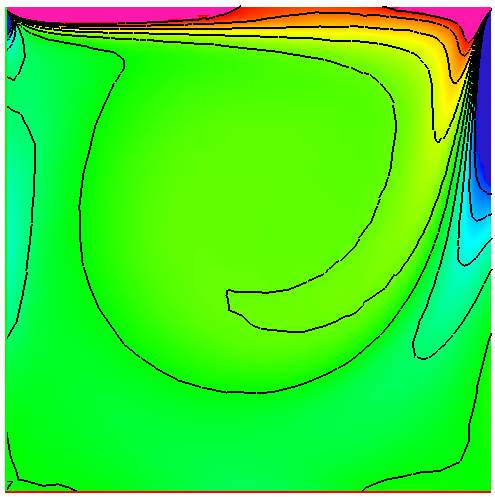
\includegraphics[width=.4\textwidth]{figs/Re500Eta10AdaptiveVorticity}
}
%$\; \vu = 0$
\end{center}

}


%%%%%%%%%%%%%%%%%%%%%%%%%%%%%%%%%%%%%%%%%%%%%%%%%%%%%%%%%%%%%%%%%%%%%
\royslide{Corner Singularities}{

Velocity boundary conditions are discontinuous at the
corners; the result is singularities in higher derivatives.
As $r \rightarrow 0$,

\vspace{-2em}
\begin{eqnarray*}
\psi(r,\theta) & = & \frac{r}{\pi^2 - 4}
\left( -\pi^2 \sin(\theta) + 2 \pi \theta \sin(\theta) + 
4 \theta \cos(\theta) \right) \\
\vorticity(r, \theta) & = & \frac{1}{(\pi^2 - 4) r}
\left( 4 \pi \cos(\theta) - 8 \sin(\theta) \right)
\end{eqnarray*}
\vspace{-2em}

}

%%%%%%%%%%%%%%%%%%%%%%%%%%%%%%%%%%%%%%%%%%%%%%%%%%%%%%%%%%%%%%%%%%%%%
\royslide{Adaptive Cavity Solution}{

\begin{center}
$\mbox{Re} = 500$, Extended Williamson fluid, 
$\nu_\infty/\nu_0 = 0.1$

\fbox{
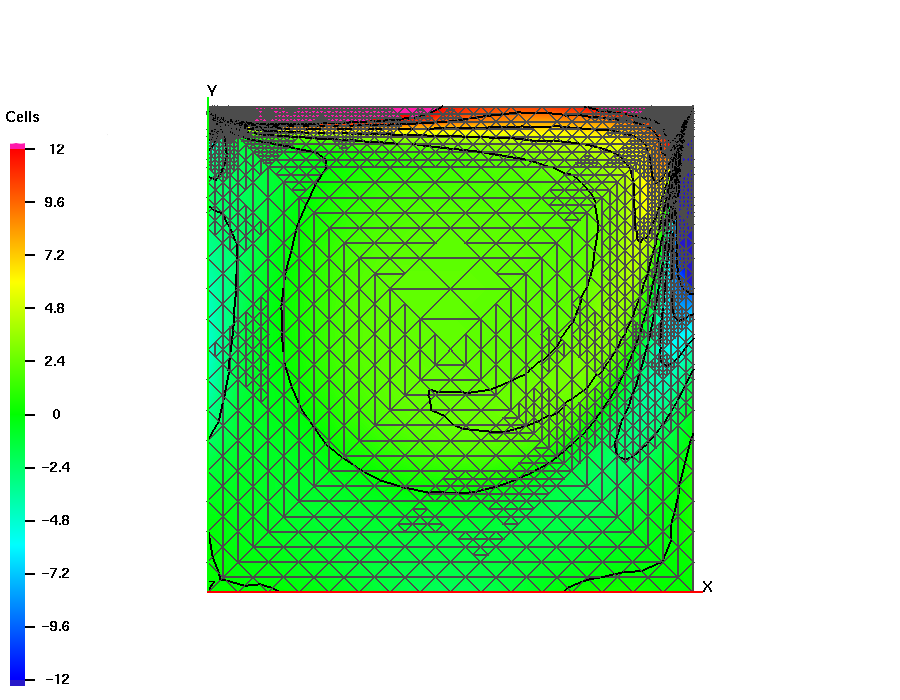
\includegraphics[width=.7\textwidth]{figs/Re500Eta10AdaptiveAll}
}
\end{center}

}


%%%%%%%%%%%%%%%%%%%%%%%%%%%%%%%%%%%%%%%%%%%%%%%%%%%%%%%%%%%%%%%%%%%%%
%\royslide{Adaptive Step Solution}{
%
%\begin{center}
%$\mbox{Re} = 0$, Newtonian fluid
%
%\fbox{
%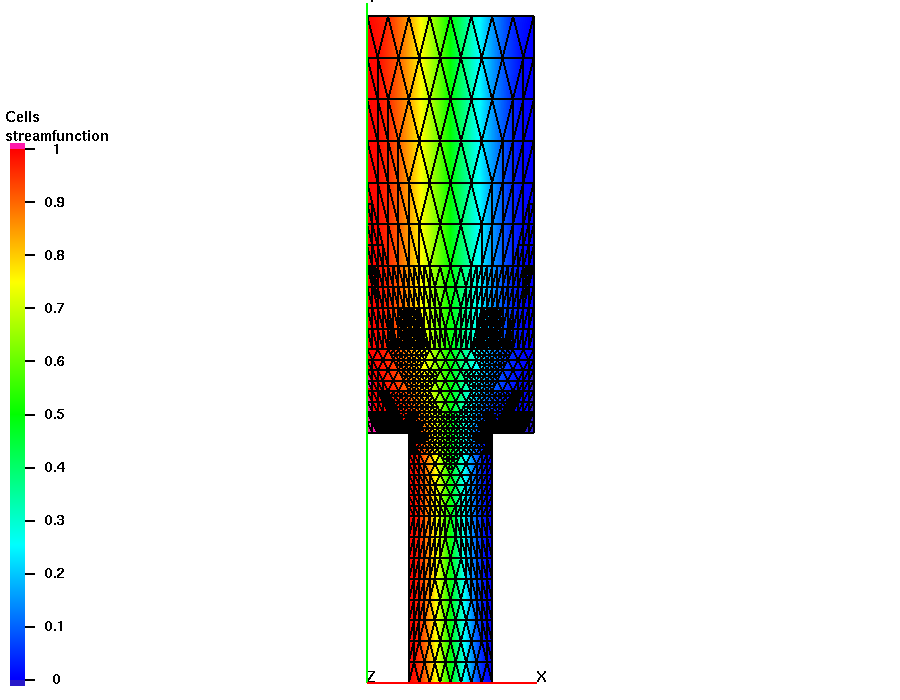
\includegraphics[width=.7\textwidth]{figs/StokesStepAll}
%}
%\end{center}
%
%}


%%%%%%%%%%%%%%%%%%%%%%%%%%%%%%%%%%%%%%%%%%%%%%%%%%%%%%%%%%%%%%%%%%%%%
%\royslide{Benchmark Convergence}{
%
%\begin{center}
%$\Delta^2 u = f$, 
%$u = \sin{xy}$
%
%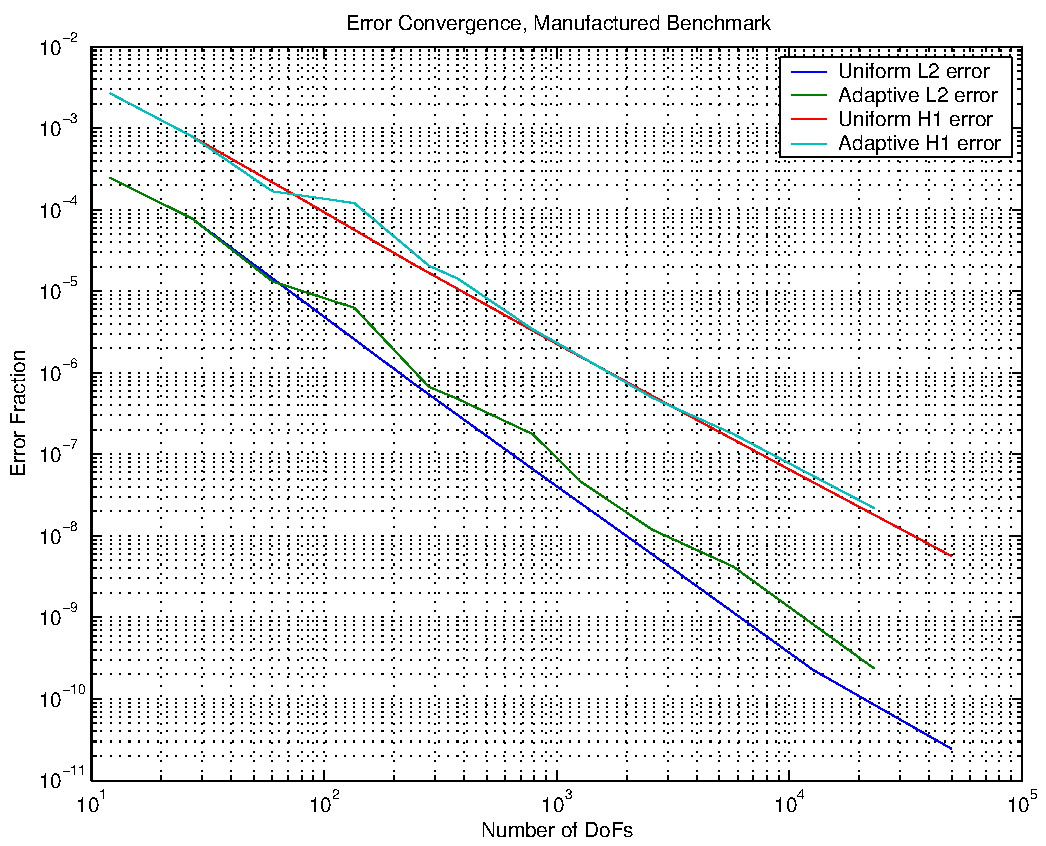
\includegraphics[width=.7\textwidth]{figs/bencherror}
%\end{center}
%
%}


%%%%%%%%%%%%%%%%%%%%%%%%%%%%%%%%%%%%%%%%%%%%%%%%%%%%%%%%%%%%%%%%%%%%%
\royslide{Driven Cavity Convergence}{

\begin{center}
$\mbox{Re} = 500$, Extended Williamson fluid, 
$\nu_\infty/\nu_0 = 0.1$

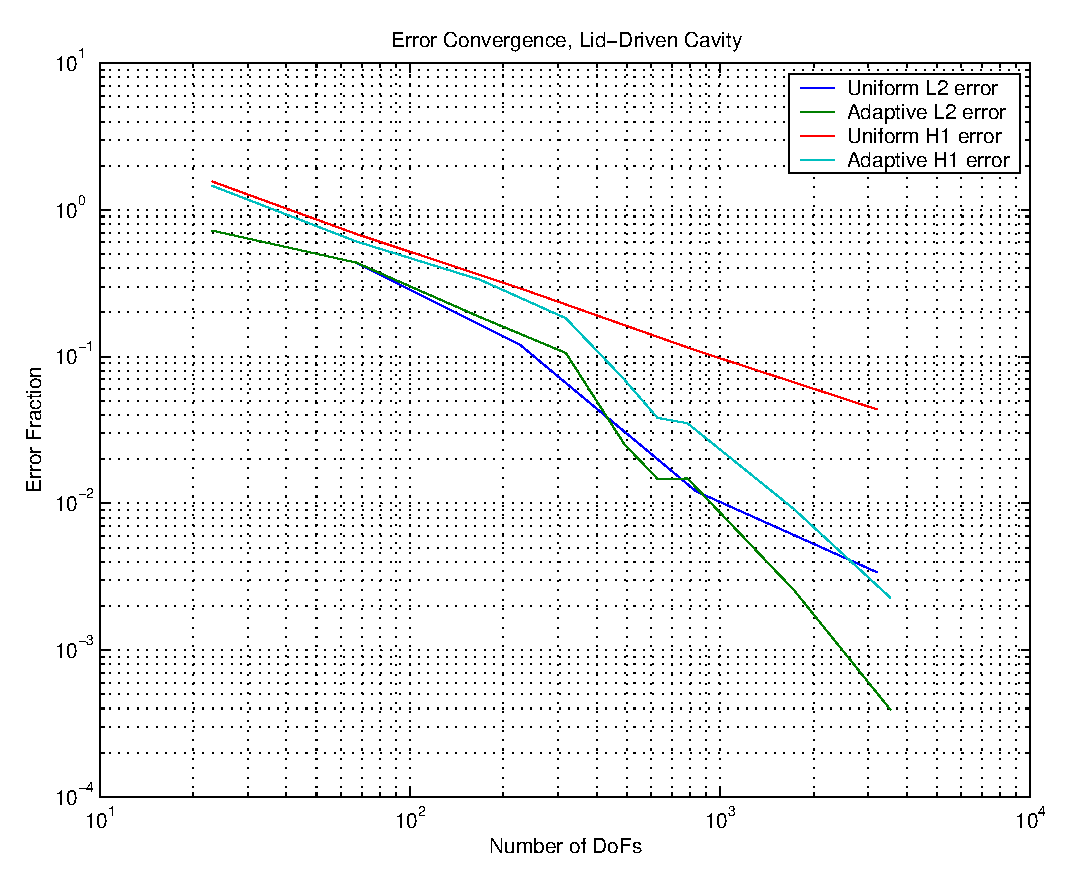
\includegraphics[width=.7\textwidth]{figs/cavityerror}
\end{center}

}

